\chapter{Dictionnaire Oracle}

\par Tous les objets (tables, vues, utilisateurs, etc.) contrôlés par le \textbf{SGBD} sont décrits dans la structure centralisée d’\textbf{ORACLE}, le dictionnaire de données.
Par conséquent, ce dictionnaire contient toutes les données nécessaires au fonctionnement du \textbf{SGBD}.
Il montre la particularité d’être directement accessible par \textbf{SQL} et d’être organisé comme une base de données de données (nous appelons cela une méta-base). 
\par Par conséquent, dans dans ce tp nous porterons une plus grande attention aux vues qui donnent accès aux tableaux des types \textbf{ALL} et \textbf{USER}.


\begin{enumerate}

    \item La méthode la plus populaire pour afficher la définition d’une table ou d’une vue est DESCRIBE, qui fournit une liste des colonnes de la table ou de la vue ainsi que des informations sur les types de données qu’ils produisent, leurs longueurs et leur nullité. Il faut entrer la commande \textbf{DESCRIBE} (or \textbf{DESC}) suivie du nom de la table ou de la vue qui nous intéresse, comme le démontre l’exemple ci-dessous:
        \begin{figure}[h]
            \centering
            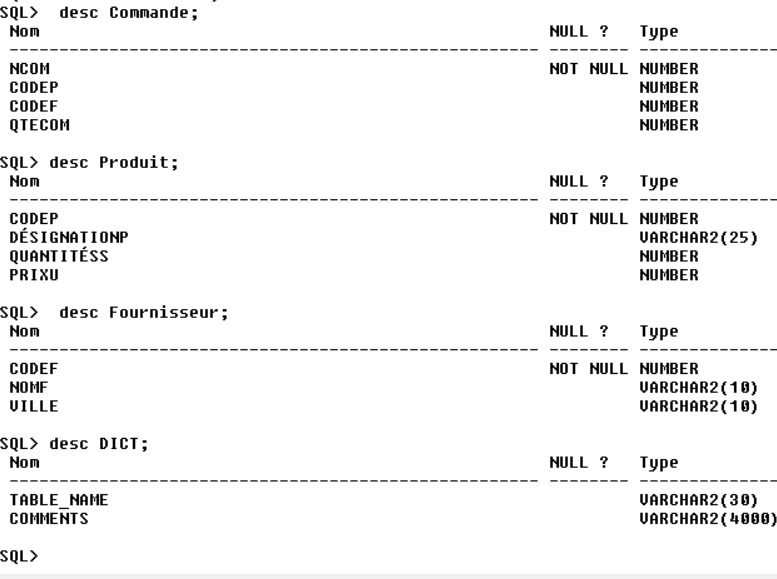
\includegraphics[width=14cm, height=8cm]{DESC.png}
            \caption{DESCRIBE }
            \end{figure}
            \\
     \par a refaire lorbanisation est le travaille progressif nécessaire pour faire évoluer un si vers une cibles (si objectif) correctement urbanisé
     \par la décomposition de l'entreprise 
     {\begin{itemize}
         \item [\textbf{1.}] Stratégie
         \item [\textbf{2.}] Métier
         \item [\textbf{3.}] fonctionnelle
         \item [\textbf{4.}] applicative
         \item [\textbf{5.}] techenique
     \end{itemize}}
     
     
    %%%%%%%%%%%%%%%%%%%%%%%%%%%%%%%%%%%%%%%%%%%%%%%%%%%%%%%%%%%%%%
    \item Le role et la structure des tables suivants :
    
        \begin{itemize}
        \item [\textbullet]\textbf{ALL\_CATALOG :}
         répertorie tous les index, tables, clusters, vues, synonymes et séquences actuellement disponibles pour l’utilisateur. Comme le démontre l’exemple ci-dessous :
            \begin{figure}[h]
            \centering
            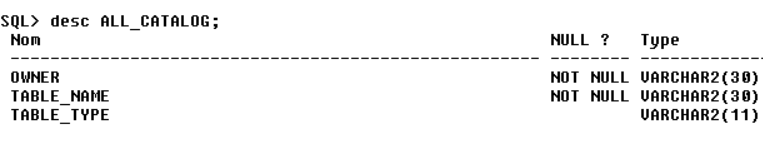
\includegraphics[width=14cm, height=7cm]{ALL_CATALOG.png}
            \caption{ALL\_CATALOG }
            \end{figure}
            %%%%%%%%%%%%%%%%%%%%%%%%%
        \item [\textbullet]\textbf{ALL\_USERS :} répertorie tous les utilisateurs qui sont actuellement visibles pour l’utilisateur dans la base de données. Comme le démontre l’exemple ci-dessous :
            \begin{figure}[h]
            \centering
            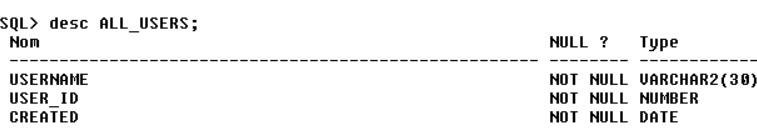
\includegraphics[width=14cm, height=7cm]{ALL_USERS.png}
            \caption{ALL USERS }
            \end{figure}
            %%%%%%%%%%%%%%%%%%%%%%%%%%%
        \item [\textbullet]\textbf{ALL\_ COL\_ COMMENTS :} affiche les commentaires sur les colonnes des tableaux et des vues accessibles à l’utilisateur actuel. Comme le démontre l’exemple ci-dessous :\\
            \begin{figure}[h]
            \centering
            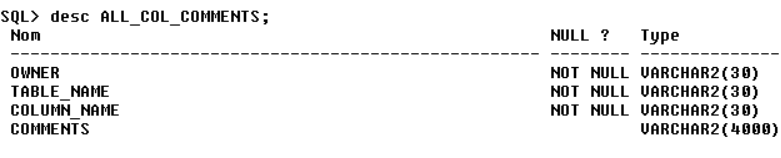
\includegraphics[width=14cm, height=7.1cm]{ALL_COL_COMMENTS.png}
            \caption{ALL COL COMMENTS }
            \end{figure}
            %%%%%%%%%%%%%%%%%%%%%%%%%%%%%
        \item [\textbullet]\textbf{ALL\_CONSTRAINTS :} describes constraint definitions on tables accessible to the current user. Comme le démontre l’exemple ci-dessous 
             \begin{figure}[h]
            \centering
            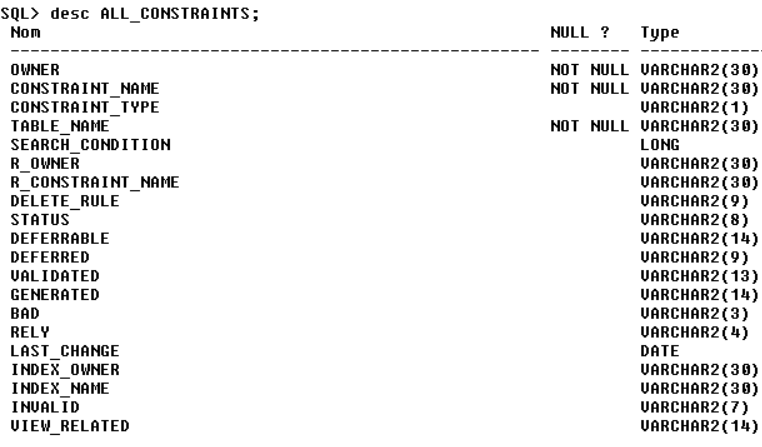
\includegraphics[width=14cm, height=7.5cm]{ALL_CONSTRAINTS.png}
            \caption{ALL CONSTRAINTS }
            \end{figure}
            \\ 
            %%%%%%%%%%%%%%%%%%%%%%%%%%%%%%
        \item [\textbullet]\textbf{ALL\_TAB\_PRIVS :} La permission d’accéder à certains objets de base de données peut être contrôlée avec des privilèges lorsque de nombreux utilisateurs y ont accès. Chaque objet a un propriétaire. Contrôle des privilèges si un utilisateur a la possibilité de modifier tout ce qui appartient à un autre utilisateur. La personne chargée d’accorder ou de révoquer les privilèges est soit l’administrateur de l’instance, soit un utilisateur disposant du privilège ADMIN, soit, dans le cas d’un objet spécifique, le propriétaire de l’objet. Comme le démontre l’exemple ci-dessous :
            \begin{figure}[h]
            \centering
            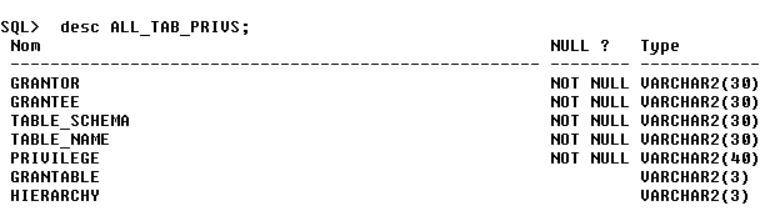
\includegraphics[width=14cm, height=7cm]{ALL_TAB_PRIVS.png}
            \caption{ALL\_TAB\_ PRIVS }
            \end{figure}
       \end{itemize}
       
    %%%%%%%%%%%%%%%%%%%%%%%%%%%%%%%%%%%%%%%%%%%%%%%%%%%%%%%%%%
    \item Le role de \textbf{USER-USER :} Elle nous aider à obtenir des informations sur l’utilisateur actuel
    (décrit l’utilisateur actuel) et contient plus de colonnes que ALL\_USERS.
    
    \par  ID de mon utilisateur est : 51
    \\
            \begin{figure}[h]
            \centering
            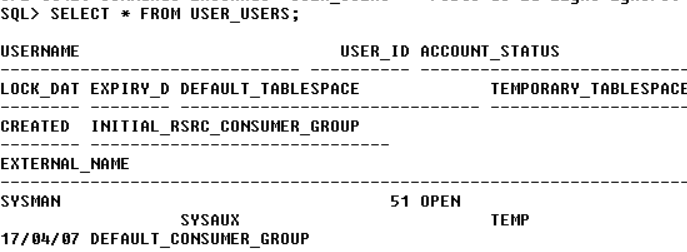
\includegraphics[width=14cm, height=5cm]{ID_UTIL.png}
            \caption{USER_USERS }
            \end{figure}
    %%%%%%%%%%%%%%%%%%%%%%%%%%%%%%%%%%%%%%%%%%%%%%%%%%
    \item La comparaison entre \textbf{ALL\_CATALOG }et\textbf{USER\_CATALOG}  :
       \begin{itemize}
           \item [\textbullet] \textbf{ALL\_CATALOG :} il nous affiche le propriétaire, nom et type de toutes les tables accessibles
           \item [\textbullet] \textbf{USER\_CATALOG :} Les vues USER contiennent des informations sur les objets appartenant au utilisateur actuel donc cette requette a pour but d'afficher le nom des tables ansi que leurs types

       \end{itemize}
    %%%%%%%%%%%%%%%%%%%%%%%%%%%%%%%%%%%%%%%%%%%%%%%%%     
    \item \textbf{USER\_TABLES} cette commande nous donne une vue globale sur toutes les tables avec leur nom, nombre de colonnes,
     informations de stockage, informations statistiques, etc.
    %%%%%%%%%%%%%%%%%%%%%%%%%%%%%%%%%%%%%%%%%%%%%%%%%%%%
    \item \textbf{USER\_TAB\_COLUMS :} cette commande nous affiche toutes les colonnes des tables et vues appartenant à l’utilisateur
    %%%%%%%%%%%%%%%%%%%%%%%%%%%%%%%%%%%%%%%%%%%%%%%%%%%%%%
    \item \textbf{USER\_CONSTRAINTS :} constraint definitions for tables 
    %%%%%%%%%%%%%%%%%%%%%%%%%%%%%%%%%%
    \item Les information sur les contrainte de type clé primaire qu j'ai crée :
          SELECT * FROM USER\_CONSTRAINTS
          WHERE CONSTRAINT\_TYPE = F\_K;

  \par se réumé va etre executer apres la connection a notre base de donées et vu que 
    
\end{enumerate}
        

